\documentclass{article}
\usepackage[utf8]{inputenc}
\usepackage{xcolor}
\usepackage{graphicx} 

% Definisci il colore per le sezioni
\definecolor{subsectioncolor}{RGB}{0, 102, 204}

% Impostazioni per la pagina
\usepackage{geometry}
\geometry{a4paper, margin=1in}

% Pacchetto per hyperlink
\usepackage{hyperref}
\hypersetup{
    colorlinks=true,
    linkcolor=blue,
    urlcolor=blue,
    citecolor=blue
}

\begin{document}
\begin{center}
    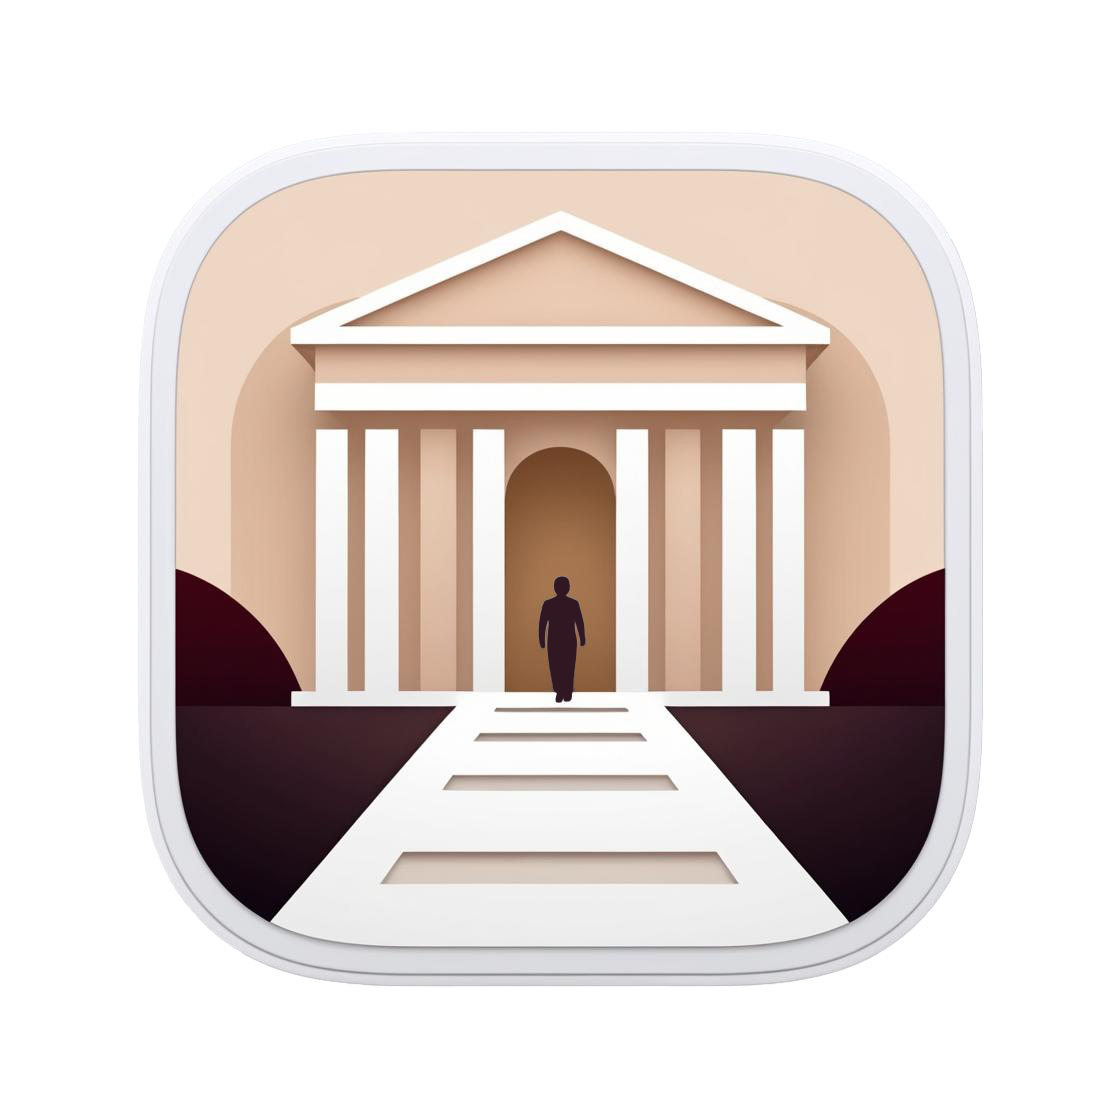
\includegraphics[width=1\textwidth]{logo.png} \\[1em]
    {\LARGE \textbf{ArtMyWay - DesignersForCulture}} \\[0.5em]
    {\Large \textbf{README del PROTOTIPO}} \\[1.5em]
    {\large 2 Dicembre 2024}
\end{center}

\section{Panoramica del Progetto}
\subsection{Introduzione}
\textbf{Membri del Team}:
\begin{itemize}
\item Alessia Franchetti-Rosada
\item Carmen Giaccotto
\item Mattia Colombo
\item Federico Previtali
\item Manoueil Michael Halim Riad Hanna
\item Valentina Petrignano
\item Michele Arrigoni
\end{itemize}
Questo progetto è stato sviluppato nell'ambito del corso \textbf{Fondamenti di Human-Computer \\ Interaction} presso il \textbf{Politecnico di Milano} per l'Anno Accademico 2024/25, sotto la supervisione della \textbf{Prof.ssa Maristella Matera}.

\subsection{Nome del Progetto}
"\textbf{\textit{ArtMyWay}}" \\
Il nome riflette il cuore del nostro obiettivo: offrire un'esperienza artistica personalizzata e su misura. È intuitivo e memorabile, e sottolinea il supporto specifico fornito agli utenti, come percorsi adattabili e audioguide personalizzate.

\subsection{Value Proposition}
"\textbf{\textit{Rendiamo l'arte un gioco da ragazzi}}"\\
\textit{ArtMyWay} si impegna a semplificare, rendere coinvolgente e accessibile l'esperienza artistica per gli \\ adolescenti. La nostra soluzione offre un'interazione tecnologica avanzata per creare un'esperienza \\ museale più attraente e personalizzata.

\subsection{Descrizione del Progetto}
\textit{ArtMyWay} è un'applicazione mobile progettata per rivoluzionare l'esperienza museale degli adolescenti. Grazie a tecnologie come la realtà virtuale e la personalizzazione, mira a:
\begin{itemize}
\item Facilitare la ricerca di musei vicini con informazioni in tempo reale sull'affluenza.
\item Offrire percorsi e audioguide personalizzate in base agli interessi e al tempo disponibile.
\item Consentire la creazione di gallerie personali digitali da condividere con altri utenti.
\end{itemize}
Il progetto nasce dall'analisi dei bisogni degli adolescenti, svolta tramite interviste e sondaggi, per \\ eliminare barriere pratiche e cognitive durante le visite museali.

\subsection{Utenti Target}
Gli utenti target principali sono adolescenti di età compresa tra i \textbf{16 e i 19 anni}. Questi giovani \\ rappresentano una fascia critica di pubblico spesso trascurata dalle esperienze museali tradizionali. \\ ArtMyWay è pensato per attrarre:
\begin{itemize}
\item Studenti liceali con interesse per l'arte e il patrimonio culturale.
\item Giovani alla ricerca di esperienze personalizzate e interattive.
\item Utenti desiderosi di un'esperienza che integri tecnologia e cultura in modo accessibile e innovativo.

\end{itemize}

\subsection{Perché una mobile app?}
\begin{itemize}
\item \textbf{Accessibilità offline} \\
Una mobile app può funzionare senza connessione a Internet, consentendo ai visitatori di accedere alle audioguide, mappe interattive e contenuti personalizzati anche in aree del museo con segnale limitato o assente.

\item \textbf{Personalizzazione avanzata} \\
Una mobile app può salvare le preferenze dell'utente, come interessi specifici, percorsi preferiti o impostazioni di lingua, offrendo un'esperienza personalizzata che si adatta alle esigenze del singolo visitatore.

\item \textbf{Interfaccia ottimizzata per l'uso in movimento} \\
Le mobile app sono progettate per essere intuitive e veloci da usare su dispositivi mobili, \\ permettendo agli utenti di navigare comodamente tra le sezioni senza dover caricare pagine web o gestire un browser.

\item \textbf{Memorizzazione locale} \\
Una mobile app può memorizzare dati come i progressi della visita o il contenuto delle audioguide, permettendo agli utenti di riascoltare o rivisitare le informazioni anche dopo aver lasciato il museo.

\item \textbf{Esperienza più immersiva} \\
Una mobile app è percepita come più coinvolgente rispetto a un sito web, dando la sensazione di un prodotto dedicato che aumenta il valore percepito dell'esperienza museale.

\end{itemize}

\subsection{Contesto di Utilizzo}
\begin{itemize}

\item \textbf{Durante la visita al museo} \\
La mobile app è utilizzata attivamente dai visitatori per:
\begin{itemize}
\item Navigare il museo: vengono fornite delle mappe che suggeriscono percorsi ottimizzati in base al tempo disponibile e alle proprie preferenze.
\item Approfondire le opere: si possono ascoltare audioguide e visualizzare contenuti aggiuntivi (es. immagini, video o descrizioni) oppure accedere a funzionalità di realtà aumentata.
\end{itemize}

\item \textbf{Pre-visita} \\
La mobile app può essere utilizzata per pianificare la visita:
\begin{itemize}
\item Creare prenotazioni: scegliere data, orario e tipo di esperienza (es. visita guidata, mostre temporanee).
\item Personalizzazione del percorso: selezionare temi o aree di interesse (arte moderna, storia antica, ecc.), creando un itinerario personalizzato.
\item Accesso a informazioni pratiche: orari di apertura, servizi disponibili, e consigli utili (es. parcheggio, accessibilità per disabili).
\end{itemize}

\item \textbf{Post-visita} \\
Dopo la visita, la mobile app può essere un mezzo per:
\begin{itemize}
\item Rivivere l’esperienza: riascoltare le audioguide, rivedere opere preferite o consultare i contenuti multimediali salvati.
\item Feedback e recensioni: lasciare recensioni sull’esperienza, valutare opere o sezioni visitate.
\end{itemize}

\end{itemize}

\section{Funzionalità dell'App e Limitazioni del Prototipo}
\subsection{Task semplice}
Dopo aver effettuato l'accesso, l'utente potrà utilizzare la funzione di ricerca per trovare musei ed \\ esposizioni in base alle proprie preferenze. L'utente avrà la possibilità di filtrare i risultati per categoria (es. Arte classica, Scienza e tecnica), valutazioni (da 1 a 5 stelle), opzioni di pagamento accettate, orario, data e zona. Inoltre, un'interessante funzione permette di verificare l'affluenza corrente nei musei tramite un indicatore percentuale. Questa informazione aiuterà l'utente a pianificare la visita in momenti meno affollati, garantendo un'esperienza più rilassante.
PS: La sezione "Selezionati per te" dell’homepage fornisce suggerimenti personalizzati basati sulle preferenze espresse durante l'uso dell'app e l’onboarding iniziale. \\
\\
\textbf{Limitazioni del prototipo}
\begin{itemize}
\item Nel prototipo la barra di ricerca non consente l'inserimento di testo e i filtri non sono interattivi.
\item Per l'onboarding viene mostrata la pagina iniziale. Non è interattiva e bisogna cliccare su "salta" per proseguire.
\item La schermata Home include la sezione 'Categoria,' che consente all’utente di selezionare una categoria di museo preferita per avviare una nuova ricerca. Tuttavia, non sono presenti schermate per visualizzare dettagli avanzati o riepiloghi dei risultati filtrati per categoria.
\item Nel prototipo, la sezione 'Selezionati per te' mostra percorsi o musei che rispecchiano i gusti degli utenti, ma non include schermate che permettano di approfondire o modificare i suggerimenti personalizzati.
\end{itemize}

\subsection{Task moderato}
L'utente potrà personalizzare la propria visita al museo in base alle proprie preferenze e al tempo disponibile. Tramite la sezione  "Personalizza la tua visita," è possibile:
\begin{itemize}
\item Selezionare la durata della visita utilizzando uno slider per adattarla al tempo a disposizione.
\item Scegliere la tipologia di percorso, tra cui: 
\begin{itemize}
\item Predefinito: un percorso suggerito standard.
\item Ordine cronologico: basato sulla sequenza temporale delle opere esposte.
\item Tematico: focalizzato su temi specifici come il Rinascimento o l’Impressionismo.
\item Secondo i tuoi interessi: personalizzato in base alle preferenze raccolte durante l’onboarding iniziale.
\end{itemize}
\item Inoltre, l’app consente di arricchire l’esperienza selezionando le opzioni Audioguida e AR/VR, che rendono la visita più interattiva e coinvolgente. Questi strumenti permettono di accedere a contenuti multimediali avanzati che accompagnano l’utente lungo il percorso scelto.
\end{itemize}
\textbf{Limitazioni del prototipo}
\begin{itemize}
\item Il percorso visibile dal prototipo è un esempio, l’obiettivo dell’applicazione rimane il voler creare percorsi diversi in base alle preferenze dell’utente.
\item Nella fase di prenotazione viene tralasciato il momento del pagamento. Nella pagina dei filtri, dove non tutti i comandi sono interattivi, si può comunque selezionare il metodo di pagamento preferito.
\end{itemize}

\subsection{Task complesso}
L’utente potrà creare e personalizzare una galleria digitale con le opere d’arte preferite visitate nei musei. Tramite la sezione "La Mia Galleria", sarà possibile:
\begin{itemize}
\item \textbf{Aggiungere opere d’arte alla galleria personale} cliccando sugli appositi pulsanti. L’applicazione riconoscerà automaticamente l’opera dalla foto caricata e la organizzerà nella galleria associata al museo visitato.
\item \textbf{Visualizzare i modelli 3D delle opere}, quando disponibili, per osservare dettagli unici e l’evoluzione delle opere nel tempo.
\end{itemize}
Dopo aver completato una visita o in un secondo momento, l’utente può \textbf{condividere} il proprio percorso culturale personalizzato. Cliccando sul simbolo della freccia nella barra inferiore destra, si \\ accede alla funzione di condivisione. È possibile scegliere tra diverse piattaforme social, come Facebook, WhatsApp, Instagram, Twitter, oppure copiare il link per condividerlo manualmente. Questa funzione consente agli utenti di mostrare le proprie esperienze museali ad amici e conoscenti, incentivando ulteriori scambi culturali.\\
\\
La sezione "\textbf{Esplora}" permette di visualizzare i percorsi e le gallerie condivisi da altri utenti della piattaforma. Gli utenti possono navigare tra le collezioni e lasciare un "Mi piace" per interagire con la community. Per accedere alla pagina "Esplora" basta cliccare sull’icona dedicata nella barra inferiore. Questa funzionalità consente di scoprire nuove esperienze museali e trarre ispirazione dai percorsi già creati e condivisi dagli altri.\\
\\
\textbf{Limitazioni del prototipo}
\begin{itemize}
\item La sezione "La mia Galleria" presenta dei tasti non interattivi per poter creare una nuova galleria o aggiungere opere ad una galleria già esistente.
\item Cliccando sul tasto "Esplora", in basso a sinistra, compare solo la pagina dei risultati non interattiva. L'obiettivo finale sarebbe quello di poter scrollare la pagina come un social, potendo mettere like e ingrandire le opere o i percorsi pubblicati dagli altri utenti dell’applicazione.
\end{itemize}

\section{Il Rapporto con i Musei Partner}
L’utilizzo e la funzionalità di questa applicazione si basano su una forte collaborazione con dei musei partner. 
Lo scopo dell’applicazione infatti è quello di poter facilitare l’esperienza museale sotto qualsiasi punto di vista: la scelta del museo, la prenotazione del biglietto, la personalizzazione della visita e molte altre cose.
Per garantire un’esperienza ottimale, i musei sono invitati a fornire materiali che arricchiscano l’applicazione, come:
\begin{itemize}
\item Immagini delle opere da includere nella galleria personale dell’utente.
\item Descrizioni dettagliate e audioguide per ciascuna opera.
\item Percorsi che prevedano l’utilizzo di visori VR durante la visita (quando disponibili).
\item Disponibilità e prezzi dei biglietti del museo.
\end{itemize}
Questa collaborazione mira a rendere l’esperienza culturale più accessibile, interattiva e coinvolgente per tutti gli utenti.

\section{Link al Prototipo}

Clicca \href{https://www.figma.com/design/DssxKU75A7I8ykLuzYvFeC/Raffinamento-Prototipo-Mobile-App?node-id=0-1\&t=XWcp3V56G4vdl11N-1}{qui} per accedere alla versione interattiva del prototipo.

\end{document}